\glsresetall
\chapter{Introduction}
\label{chap:introduction}

This document presents the \textit{Master Thesis} in \textit{Informatics Engineering} of the student \textit{André Pascoal Bento's} during the school year of 2018/2019, taking place in the \textit{\gls{dei}}, \textit{Faculty of Sciences and Technology} of the \textit{University of Coimbra}.

\section{Context}
\label{sec:context}

%In today's world, software systems tend to become more distributed, resulting in new approaches that lead to new solutions and new patterns of developing software. One way to solve this is to develop systems that have their components decoupled, creating software with ``small pieces'' connected to each other encapsulating and providing a specific function in the larger service. This way of developing software is called Microservices and has become mainstream in the enterprise software development industry~\cite{Dragoni2017}. However, with this kind of approach, the systems complexity is increased as a whole because with more ``small pieces'', more connections are needed and with this more problems related to latency and requests become harder to detect, analyse and correct~\cite{DiFrancesco2017}.

Software systems are becoming larger and more distributed than ever, thus requiring new solutions and new development patterns. One approach that emerged in recent years is to decouple large monolithic components into interconnected ``small pieces'' that encapsulate and provide specific functions. These components are known as ``Microservices'' and have become mainstream in the enterprise software development industry~\cite{Dragoni2017, microservices_definition}. Besides their impact on latency, fine-grained distributed systems, including microservices, increase system complexity, thus turning anomaly detecting into a more challenging task~\cite{Francesco2017}.

%To keep a history of the work performed by this kind of systems, multiple techniques like monitoring~\cite{Joyce1987}, logging~\cite{logging} and tracing~\cite{distributed_tracing} are adopted. Monitoring consists on measuring some aspects like \gls{cpu} usage, hard drive usage and network latency of the entire system or of some specific node in a distributed system. Logging provides an overview to a discrete, event-triggered log. Finally, tracing is much similar to logging, however the focus is  registering the flow of execution of the program through several system modules and boundaries. Lastly, distributed tracing, shares the focus on preserving causality relationships, however, is geared towards the modern distributed environments, where state is partitioned over multiple, threads, processes, machines and even geographical locations. This last one is better explained in Subsection~\ref{subsec:distributed_tracing} - \nameref{subsec:distributed_tracing}. There are multiple approaches to gather information of this kind of systems, each with its benefits and disadvantages.

To tackle this problem, \gls{devops} resort to techniques like monitoring~\cite{monitoring}, logging~\cite{logging}, and end-to-end tracing~\cite{distributed_tracing}, to observe and maintain records of the work performed in a microservices system. Monitoring consists of measuring aspects like \gls{cpu} and hard drive usage, network latency and other infrastructure metrics around the system and components. Logging provides an overview to a discrete, event-triggered log. Tracing is similar to logging, but focuses on registering the flow of execution of the program, as requests travel through several system modules and boundaries. Distributed tracing can also preserve causality relationships when state is partitioned over multiple threads, processes, machines and even geographical locations. Subsection~\ref{subsec:distributed_tracing} - \nameref{subsec:distributed_tracing}.

The main problem with this is that there are not many implemented tools for processing tracing data and none for performing analysis of this type of data. For monitoring it tend to be easier, because data is represented in charts and diagrams, however for logging and tracing it gets harder to manually analyse the data due to multiple factors like its complexity, plethora and increasing quantity of information. There are some visualisation tools for the \gls{devops} to use, like the ones presented in Subsection~\ref{subsec:distributed_tracing_tools}~-~\nameref{subsec:distributed_tracing_tools}, however none of them gets to the point of analysing the system using tracing, has they tend to be developed only for visualisation and display of tracing data in a more human readable way. Distributed tracing data can be used by \gls{devops} because it is particularly well-suited to debugging and monitoring modern distributed software architectures, such as microservices. This kind of data contains critical information about request paths, response time and status, services presented in the system and their relationship and, for this reason, can be further analysed to detect anomalous behaviours in requests, response times and services in these systems. Nevertheless, this is critical information about the system behaviour, and thus there is the need for performing automatic tracing analysis.

\section{Motivation}
\label{sec:motivation}

Exploring and develop ways to perform tracing analysis in microservice based systems lay down the motivation behind this work. The analysis of this kind of systems tend to be very complex and hard to perform due to their properties and characteristics, as it is explained in Subsection~\ref{subsec:microservices} - \nameref{subsec:microservices}, and to the type of data to be analysed, presented in Subsection~\ref{subsec:distributed_tracing} - \nameref{subsec:distributed_tracing}.

\gls{devops} teams have lots of problems when they need to identify and understand problems with distributed systems. They usually detect the problems when a client complains about the quality of service, and after that, \gls{devops} dive in monitoring metrics like, e.g, \gls{cpu} usage, usage, hard drive usage and network latency. Later on, they use distributed tracing data visualisations and logs to find some explanation to what is causing the reported problem. This involves a very hard and tedious work of look-up through lots of data that represents the history of work performed by the system and, in most cases, this tedious work reveals like a big ``find a needle in the haystack'' problem. For this reason, \gls{devops} have hard time finding problems in services and end up ``killing'' and rebooting services, which can be bad for the whole system. However, due to lack of time and difficulty in identifying anomalous services precisely this is the best approach to perform.

Problems regarding the system operation are more common in distributed systems and their identification must be simplified. This need of simplification comes from the exponential increase in the amount of data needed to retain information and the increasing difficulty in manually managing distributed infrastructures. The work presented in this thesis, aims to perform a research around these needs and focus on presenting some solutions and methods to perform tracing analysis.

\section{Goals}
\label{sec:goals}

The main goals for this thesis consist on the main points exposed bellow:

\begin{enumerate}
    \item Search for existing technology and methodologies used to help \gls{devops} teams in their current daily work, with the objective of gathering the best practices about handling tracing data. Also, we aim to understand how these systems are used, what are their advantages and disadvantages to better know how we can use them to design and produce a possible solution capable of performing tracing analysis. From this we expect to learn the state of the field for this research, covering the core concepts related work and technologies, presented in Chapter~\ref{chap:state_of_the_art}~-~\nameref{chap:state_of_the_art}.
    \item Perform a research about the main needs of \gls{devops} teams, to better understand what are their biggest concerns that lead to their approaches when performing pinpointing of microservices based systems problems. Relate these approaches with related work in the area, with the objective of understanding what other companies and groups have done in the field of automatic tracing analysis. The processes used to tackle this type of data, their main difficulties and conclusions provide a better insight about the problem. From this we expected to have our research objectives clearly defined and a compilation of questions to be evaluated and answered, presented in Chapter~\ref{chap:research_objectives_and_approach}~-~\nameref{chap:research_objectives_and_approach}.
    
    \item Reason about all the information gathered to design and produce a possible solution that provides a different approach to perform tracing analysis. From this we expect first to propose a possible solution, presented in Chapter~\ref{chap:proposed_solution}. Then we implemented it using state of the art technologies, feed it with tracing data provided by Huawei and collect results, presented in Chapters~\ref{chap:implementation_process}~-~\nameref{chap:implementation_process} and \ref{chap:results_analysis_and_limitations}~-~\nameref{chap:results_analysis_and_limitations}. Finally, we provide conclusions to this research work in Chapter~\ref{chap:conclusion_and_future_work}~-~\nameref{chap:conclusion_and_future_work}.
\end{enumerate}

\section{Work Plan}
\label{sec:work_plan}

%The methodology of work carried out in this research project is presented in this chapter. First, every member involved will be mentioned as well as their individual contribution for the project. Second, the adopted approach and organisation process of the collaborators involved will be explained. Finally, the work plan including foreseen and real work plans for the whole year are presented and discussed.

%The main people involved in this project were myself, André Pascoal Bento, student at the Master course of Informatics Engineering at \gls{dei}, who carried out the investigation and development of the project. In second, Prof. Filipe Araújo, assistant professor at the University of Coimbra, who contributed with his vast knowledge and guidance on topics about distributed systems and cloud computing. In third, Prof. Jorge Cardoso, Chief Architect for Intelligent CloudOps at Huawei Technologies, who contributed with his vision, great contact with the topics addressed in this work and with the tracing data set from Huawei Cloud Platform~\cite{huawei_cloud_platform}. In fourth, Eng. Jaime Correia, doctoral student at \gls{dei}, who contributed with his vast technical knowledge regarding the topics of tracing and monitoring microservices. In Sixth, Eng. Ricardo Filipe, doctoral student at \gls{dei}, who contributed with peer review of the paper submitted to the International Symposium on Network Computing and Applications (IEEE NCA 2019).
% , like the ones mentioned before,

This work represents an investigation and was mainly an exploratory work, therefore, no development methodology was adopted. Meetings were scheduled to happen every two weeks. We gathered with the objective of discussing the work carried out and define new courses of research. The main focus in the first semester were topics like published papers, state of the art, analysis of related work and a proposition of solution. In the second semester, two more colleagues joined the project (DataScience4NP) and started participating in meetings, which contributed with wider discussions of ideas. In these meeting, the main topics covered were: implementation of the proposed solution, research for algorithms and methods for trace processing and analysis of gathered data. In the end, these meetings were more than enough to keep the productivity and good work.

Total time spent in each semester, by week, were sixteen $(16)$ hours for the first semester and forty $(40)$ hours for the second. In the end, it was spent a total of three-hundred and four $(304)$ hours for the first semester, starting in $11.09.2018$ and ending in $21.01.2019$ $(19$ weeks $*$ $16$ hours per week$)$. For the second semester, eight-hundred and forty $(840)$ hours were spent, starting in $04.02.2019$ and ending in $28.06.2019$ $(21$ weeks $*$ $40$ hours per week$)$.

%Before starting this research project, there was a work plan defined for two semesters presented in the proposition. For purposes of analysis and comparison, these plans, proposed and real of both semesters, are presented in Figures~\ref{fig:proposed_work_plan_semester_1_and_2} and~\ref{fig:real_work_plan_semester_1}.

As we can see in Figures~\ref{fig:proposed_work_plan_semester_1_and_2} and~\ref{fig:real_work_plan_semester_1}, the proposed work for the first semester has suffered changes, when comparing it to the real work plan. Task 1 - Study the state of the art (Fig.~\ref{fig:proposed_work_plan_semester_1_and_2}), was branched in two, 1 - Project Contextualisation and Background and 2 - State of the Art, however, these last ones tocked more time to accomplish due to lack of work in the field of trace processing and trace analysis, core topics for this thesis. Task 2 - Integrate the existing work (Fig.~\ref{fig:proposed_work_plan_semester_1_and_2}) was replaced by task 3 - Prototyping and Technologies Hand-On (Fig.~\ref{fig:real_work_plan_semester_1}) due to redirections in the work course. This redirection was done due to interest increase in testing state of the art technologies, allowing us to get a better visualisation of the data provided by Huawei and enhancing our investigation work. The remaining tasks took almost the predicted time to accomplish.

For the second semester, an ``expected'' work plan was defined with respect to the proposed work, presented in Figure~\ref{fig:proposed_work_plan_semester_1_and_2}, and the state of the research at the time. The expected work plan can be visualized in Figure~\ref{fig:complete_work_plan_semester_2}. This Figure contains the expected (Grey) and real (Blue) work for the second semester.

%To estimate the effort for each task, we decided to: First, group tasks in four groups depending on complexity and work load. Second, discuss if they were in the right group taking into consideration what is defined in the solution and the task background knowledge. Third, assign the defined values to each group. This values represent the work days for each task, and in this case we defined the following four: 3(three), 5(five), 8(eight) and 12(twelve) working days as they are akin to the Fibonacci suites~\cite{project_estimation_times}. The only task that were not submitted to this, was the task 3 - Write the final report.

Three main changes were made over time in the work plan. The first one involved a reduction in task 1 - Metrics collector tool. When the solution was being implemented and the prototype was capable to extract a set of metrics, we decided to stop the implementation process to analyse the research questions. Second, this analysis lead to an emergence of ideas, ``2 - Restructuring research questions',' and thus a project redirection. Tests were removed from planning and the project followed with the objective of producing the data analyser, ``3 - Data Analyser tool'', and with it, answer two main questions regarding anomalous services and quality of tracing. Third, the introduction of a new task, ``4 - Write paper to NCA 2019'', covering the work presented in this thesis.

%These Figures have been created by an open-source tool called GanttProject~\cite{gantt_project_tool} that produce Gantt charts, a kind of diagram used to illustrate the progress of the different stages of a project.

\begin{landscape}
    \begin{figure}
        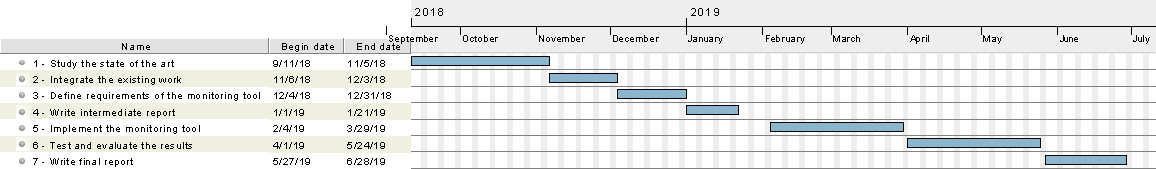
\includegraphics[height=0.234\textwidth]{images/proposed_work_plan_semester_1_and_2.pdf}
        \caption{Proposed work plan for first and second semesters.}
        \label{fig:proposed_work_plan_semester_1_and_2}
        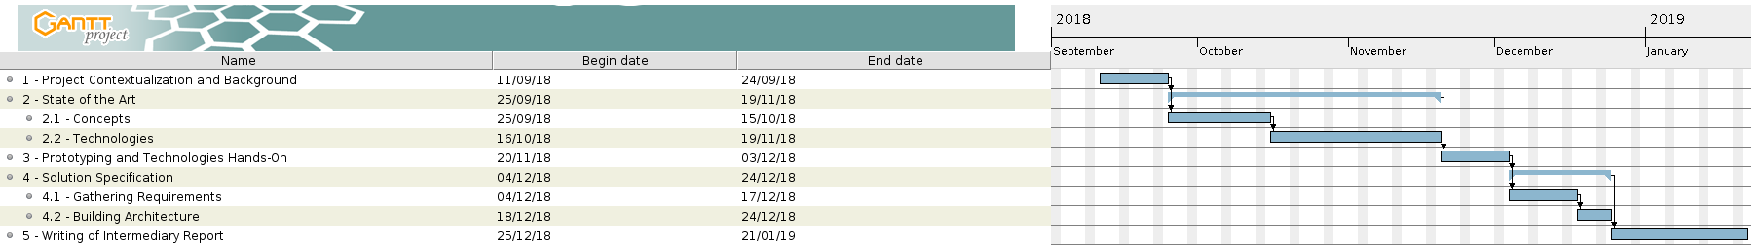
\includegraphics[height=0.3\textwidth]{images/real_work_plan_semester_1.pdf}
        \caption{Real work plan for first semester.}
        \label{fig:real_work_plan_semester_1}
    \end{figure}
\end{landscape}

\begin{landscape}
    \begin{figure}
        %\includegraphics[width=1.0\textwidth]{Image.eps}
        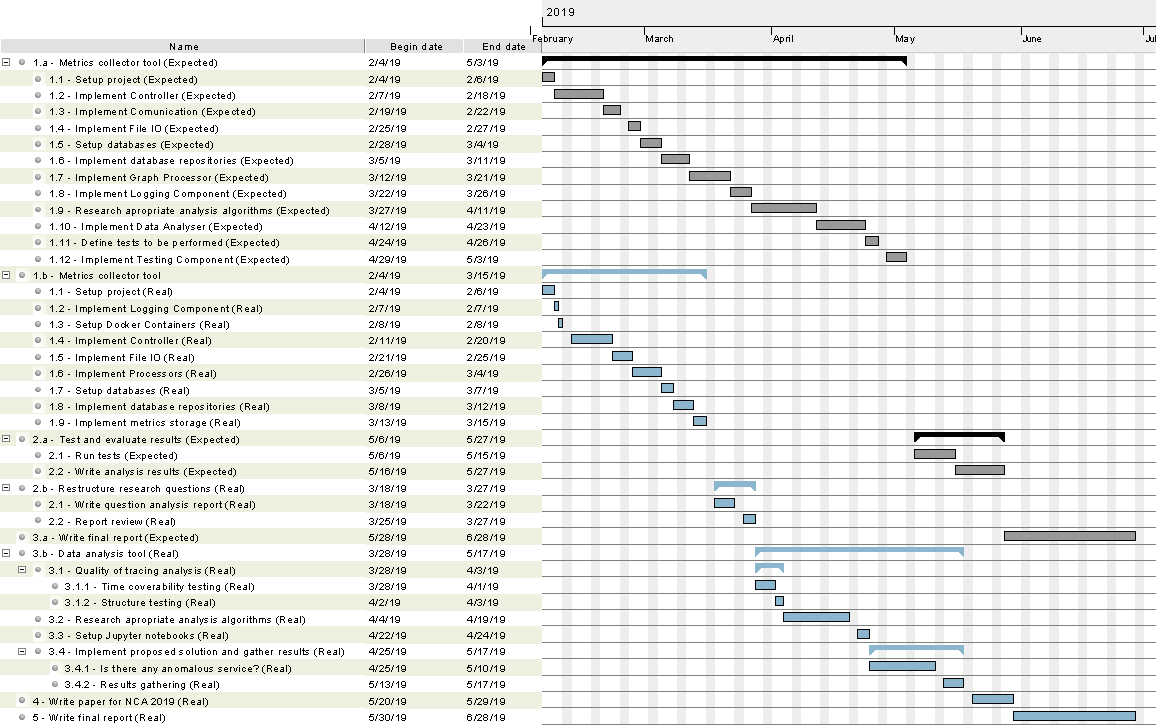
\includegraphics[height=1.0\textheight]{images/complete_work_plan_semester_2.pdf}
        \caption{Real and expected work plans for second semester.}
        \label{fig:complete_work_plan_semester_2}
    \end{figure}
\end{landscape}

\section{Research Contributions}
\label{sec:research_contributions}

From the work presented on this thesis, the following research contribution were made:

\begin{itemize}
    \item Andre Bento, Jaime Correia, Ricardo Filipe, Filipe Araujo and Jorge Cardoso. On the Limits of Automated Analysis of OpenTracing. International Symposium on Network Computing and Applications (IEEE NCA 2019). 
    %(The paper is waiting review)
\end{itemize}

\section{Document Structure}
\label{sec:document_structure}

This section presents the document structure in this report, with a brief explanation of the contents in every section. This document contains a total of eight chapters, including this one, Chapter~\ref{chap:introduction}~-~\nameref{chap:introduction}. The remaining six are presented as follows:

\begin{itemize}
    %\item In Chapter~\ref{chap:methodology}~-~\nameref{chap:methodology} the elements involved in this work, with their contributions, as well as the work plan, with ``foreseen'' and ``real'' work plans comparison and analysis are presented.
    \item In Chapter~\ref{chap:state_of_the_art}~-~\nameref{chap:state_of_the_art} the current state of the field for this kind of problem is presented. This chapter is divided in three sections. The first one, Section~\ref{sec:concepts}~-~\nameref{sec:concepts} introduces the reader to the core concepts to know as a requirement for a full understanding of the topics discussed in this thesis. The second, Section~\ref{sec:technologies}~-~\nameref{sec:technologies} presents the result of a research for current technologies, that are able to help solving this problem and produce a proposed solution to be implemented. Finally, Section~\ref{sec:related_work}~-~\nameref{sec:related_work} presents the reader to related researches produced in the field of distributed tracing data handling.
    \item In Chapter~\ref{chap:research_objectives_and_approach}~-~\nameref{chap:research_objectives_and_approach} the problem is approached in detail and the objectives of this research are presented. This chapter is divided in two sections. First, Section~\ref{sec:problem_definition}~-~\nameref{sec:problem_definition}, provides a concrete definition of the problem, how we tackled it, the main difficulties that were found and the objectives involved in order to propose a solution. Second, Section~\ref{sec:research_questions}~-~\nameref{sec:research_questions}, a compilation of questions are presented and evaluated with some reasoning about possible ways to answer them.
    \item In Chapter~\ref{chap:proposed_solution}~-~\nameref{chap:proposed_solution} a possible solution for the presented problem is exposed and explained in detail. This chapter is divided in four sections. The first one, Section~\ref{sec:functional_requirements}~-~\nameref{sec:functional_requirements}, expose the functional requirements with their corresponding priority levels and a brief explanation to every single one of them. The second one, Section~\ref{sec:quality_attributes}~-~\nameref{sec:quality_attributes}, contains the gathered non-functional requirements that were used to build the solution architecture. The third one, Section~\ref{sec:technical_restrictions}~-~\nameref{sec:technical_restrictions}, presents the defined technical restrictions for this project. The last one, Section~\ref{sec:architecture}~-~\nameref{sec:architecture}, presents the possible solution architecture using some representational diagrams, and ends with an analysis and validation to check if the presented architecture meets up the restrictions involved in the architectural drivers.
    \item In Chapter~\ref{chap:implementation_process}~-~\nameref{chap:implementation_process}, the implementation process of the possible solution is presented with detail. This chapter is divided in three main sections covering the whole implementation process, from the input data set through the pair of components presented in the previous chapter. The first one, Section~\ref{sec:huawei_tracing_data_set}~-~\nameref{sec:huawei_tracing_data_set}, the tracing data set provided by Huawei to be used as the core data for research is exposed with some detail. Second, in Section~\ref{sec:open_tracing_processor_component}~-~\nameref{sec:open_tracing_processor_component} we present the possible solution for the first component, namely ``Graphy \gls{otp}'', that processes and extracts metrics from tracing data. The final Section~\ref{sec:data_analysis_component}~-~\nameref{sec:data_analysis_component} presents the possible solution for the second component, namely ``Data Analyser'', that handles data produced by the first component and produces the analysis reports. Also, in the last two sections presented, the used algorithms and methods in the implementations are properly detailed and explained.
    \item In Chapter~\ref{chap:results_analysis_and_limitations}~-~\nameref{chap:research_objectives_and_approach}, the gathered results, corresponding analysis and limitations of tracing data are presented. This chapter is divided in three main sections. The first one, Section~\ref{sec:anomaly_detection}~-~\nameref{sec:anomaly_detection}, the results regarding the gathered observations on the extracted metrics of anomalous service detection are presented and explained. Second, in Section~\ref{sec:trace_quality_analysis}~-~\nameref{sec:trace_quality_analysis} the results obtained from the quality analysis methods applied to the tracing data set are presented and explained. The final Section~\ref{sec:limitations_of_opentracing_data}~-~\nameref{sec:limitations_of_opentracing_data} we present the limitations felted when designing a solution to process tracing data, more precisely OpenTracing data.
    \item Last, in Chapter~\ref{chap:conclusion_and_future_work}~-~\nameref{chap:conclusion_and_future_work}, the main conclusions for this research work are presented. To present this chapter, a reflection about the implemented tools, methods produced and the open paths from this research are exposed. Also a reflection of the main difficulties felted with this research regarding the handling of tracing data are presented. After this, the future work that can be addressed, considering this work, is properly explained.
\end{itemize}

%Next, Chapter~\ref{chap:methodology} - \nameref{chap:methodology}, the elements involved in this work, their contributions and work plans for this research project are presented.

Next, Chapter~\ref{chap:state_of_the_art}~-~\nameref{chap:state_of_the_art}, the state of the field is covered with core concepts, technologies and related work.

\checkoddpage
\ifthenelse{\boolean{oddpage}}
{
    \newpage
    \blankpage
}
{
    % Even page
}